% Chapter 4
\chapter{Graph Kernels} % Main chapter title

\label{Chapter4} % For referencing the chapter elsewhere, use \ref{Chapter1} 

\lhead{Chapter4. \emph{Graph Kernels}} % This is for the header on each page - perhaps a shortened title

%----------------------------------------------------------------------------------------
Kernels methods offer natural framework to study machine learning questions in different field, where graphs are used to model relationships between structure, with nodes representing objects and edges the relations between them. In this scenario, researcher direction leads to one important questions: “How similar are two graphs to each other?". To answer the above question, the kernels between graph was first proposed by G{\"a}rtner et al. \citep{Gartner2003} and later extended by Borgwardt et al.\citep{Borgwardt2005}. The graph kernels replace the explicit projection in feature space with the evaluation of a symmetric semi-definite positive similarity function. It can utilize infinite possible feature spaces by the learning algorithm with complexity of the kernel function, rather on the size of the feature space. Most kernel functions for graphs associate specific types of substructures to features, so the evaluation is then related to the number of common substructures between two graphs. The most common substructures widely used in the literature includes include random walks, paths, tree structures and rational kernels \citep{Vishwanathan2010}. Now, we review some of the representative graph kernels. 

\section{Random Walk Graph Kernels}
\label{sec:RWGK}

One of the popular graph kernel, random walk graph kernel \citep{Gartner2003, Kashima2003} counts matching walks in two input graphs. The basic idea behind this kernel to perform simultaneous random
walks between the vertexes of the graphs,  given a pair of graphs and count the number of matching paths.

\subsection{Computation}

Taking two graph $G_{1}, G_{2}$, let $E_{\times}$ denote the adjacency matrix
of their direct product $E_{\times} = E (G1 \times G2) $, and $V_{\times}$ denote the vertex set of the direct product  $V_{\times} = V (G1 \times G2) $. With a sequence of weights $\lambda = \lambda_{0}, \lambda_{1},...$
($\lambda_{i} \in R$; $\lambda_{i} \geq 0$ for all $i \geq N$) the direct product kernel is defined as:

%
\begin{equation}
K_{\times} (G_{1}, G_{2}) = \displaystyle\sum_{i,j=1}^{| V_{\times} |} \Bigg[ \displaystyle\sum_{k=0}^{\infty} \lambda_{k}E_{\times}^{k} \Bigg]_{ij}
\end{equation}
%

The graph kernel $K(G_{1}, G_{2})$ is computed efficiently computing matrix power series $\lim_{n \to \infty} \sum_{i=0}^{n} \lambda_{i}E^{i}$, which is explained in  Gartner et al. \citep{Gartner2003} by taking exponential and geometric series. The graph kernel is normalised to get similarity index in our case. In simple words, elegant computation involves, computing walk of length k by looking at the $k^{th}$ power of the adjacency matrix, then constructing direct product of the graph $G_{1}, G_{2}$ and counting walk on the product graph $K_{\times} (G_{1}, G_{2})$.  $E^{k} (i,j)$ = $c$ means that $c$ walks of length $k$ exist between vertex $i$ and vertex $j$. 

\subsection{Disadvantages}
Although random walk kernels and path based kernels
are still among the widely adopted graph kernels, It is prohibitively expensive, requiring $O(n_{6})$ runtime and suffers 
from the problem of tottering \citep{Mahe2004} and halting \citep{Sugiyama2015}. Other common disadvantage with them is that walks and paths do not capture information of the substructures present in the graph.

\subsection{Potential solutions}

The computation of the above was greatly improved by Vishwanathan et al. \citep{Vishwanathan2010} using iterative methods, including those based on Sylvester equations, conjugate gradients, and fixed-point iterations. Other improvements by Kang et al. \citep{Kang2012} takes account for just unlabeled graphs with the normalized weight matrix. Tottering problem was solved by  Mahe et al.\citep{Mahe2004} by doing special transformation on the input graphs, but it suffer from adverse computation time ($O(n)$ to $O(n_{2}$) and does not show a uniform improvement of classification accuracy. Replacing walk by path  Borgwardt et al.\citep{Borgwardt2005}, solved the tottering and  halting problem, but dense matrix representation for connected graphs, may lead to memory problems on large graphs. 

But the recent paper by  Sugiyama and Borgwart \citep{Sugiyama2015} claimed geometric random walk kernels suffers from the problem  referred to as halting: Longer walks are downweighted so much that the similarity score is completely dominated by the comparison of walks of length 1. This means that defining kernels for the graph is ongoing process, which keeps the improvements cycles on.

\section{Shortest Path Kernel on Graphs}

The foundation of shortest path graph kernels emerged because, paths do not suffer from tottering, as the number of self-loop-avoiding paths between all pairs of nodes of a given graph is useful for understanding the structure of the graph. But computing the number of such paths between all nodes is however a computationally hard task. Instead, only the number of shortest paths is counted  between node pairs in polynomial time avoiding cycles, thus is used as best structural measure in graph kernels \citep{Kriegel2005}.

\subsection{Methodology}
The first steps involves computing all-pairs-shortest-paths for $G_{1}$ and $G_{2}$ via Floyd-Warshall or Dijkstra’s algorithm. We then define graph kernel as a function $k(G_1,G_2)$ on pairs of graphs, which can be represented as an inner product $k(G_1,G_2) = \langle \phi(G_1), \phi(G_2) \rangle_{\mathcal{H}}$ for some mapping $\phi(G)$ to a Hilbert space $\mathcal{H}$, of possibly infinite dimension. Denoting $D(G)$ as the multi set of shortest distances between all node pairs in the graph $G$, we define  shortest path kernels two given graphs $G_1$ and $G_2$ as:

%
\begin{align}
K_{\rm SP}(G_{1}, G_{2})
=\sum_{d_1\in D(G_{1})}\;\sum_{d_2\in D(G_{2})}k(d_1,d_2),
\label{eq:SPKernel}
\end{align}
%
where $k$ is a positive definite kernel \citep{Borgwardt2005, Kriegel2005}.

\subsection{Advantages}
The shortest path graph kernels doesn't suffer  from tottering, and has  better accuracy on classification benchmarks. Runtime is in $O(n_{4})$, which includes computing all-pairs-shortest-paths for $G_{1}$ and  for $G_{2} \colon O(n_{3})$. Also, comparing all pairs of shortest paths from $G_{1}$ and  $G_{2} \colon O(n_{4})$. It is empirically faster than (fast) random walk kernels (probably due to graph size) \citep{Kriegel2005}.

\subsection{Disadvantages}

The complexity of order $O(n_{4})$  is too slow for large graphs. The essential step, dense matrix representation for connected graphs, may lead to memory problems on large graphs.

\subsection{Potential Solution}

The above problem of dense matrix representation was solved by new tree-based kernel for graphs \citep{Martino2012}. Graphs are decomposed into multisets of ordered Directed Acyclic Graphs (DAGs) and a family of kernels computed by application of tree kernels extended to the DAG domain. They provide richer representation of graph structure than walk-based approach, but their runtime grows exponentially with the recursion depth of the tree.

\section{Graphlet Kernels}
While using graph kernels, a practitioner is faced with some important dilemmas: Which graph kernels to be chosen for particular application?
If chosen, how good it capture graph similarity by being better
than others?  Is it cheap to compute? Unfortunately, all the above questions are too difficult to be answered, and no theoretical justification supports the selection of particular graph kernels.\citep{Yanardag2015B}.

The one way to look into the solutions of the above problem is efficiently computable representation that adequately captures the topology of the input graphs. Graph kernels do it by counting on the distribution of subgraphs of size $k$, refereed to as "graphlets".

\subsection{Description}

Using the notation from Yanardag and Vishwanathan paper \citep{Yanardag2015B}, we define graph as pair $G=(V,E)$ where $V = \left \{ v_1, v_2, \ldots,
  v_{|V|} \right \}$ is an ordered set of \emph{vertices} or
\emph{nodes} and $E \subseteq V \times V$ is a set of \emph{edges}.
Given $G = (V, E)$ and $H = (V_H , E_H )$, $H$ is a {\em sub-graph} of
$G$ iff there is an injective mapping $\alpha : V_H \rightarrow V$ such
that $(v, w) \in E_H$ iff $(\alpha(v), \alpha(w)) \in E$.  Two graphs $G
= (V, E)$ and $G' = (V', E')$ are {\em isomorphic} if there exists a
bijective mapping $g: V \rightarrow V'$ such that $(v_i, v_j) \in E$ iff
$(g(v_i), g(v_j)) \in E'$. {\em Graphlets} are small, connected,
non-isomorphic sub-graphs of a large network.

With clear notation, we now define graphlet kernels. Let $\mathcal{G}_{k} = \{ g_{1}, g_2, \ldots, g_{n_k} \}$ be the set of
size-$k$ graphlets where $n_k$ denotes the number of unique graphlets of
size $k$.  Given a graph $G$, we define $f_{G}$ as a normalized vector
of length $n_k$ whose $i$-th component corresponds to the frequency of
occurrence of $g_{i}$ in $G$:
%
\begin{align}
  \label{eq:gk}
  f_G = (\frac{c_1}{\sum_{j}^{n_k} c_j}, \cdots, \frac{c_{n_k}}{\sum_{j}^{n_k} c_j})^T.
\end{align}
%
Here $c_i$ denotes number of times $g_i$ occurs as a sub-graph of
$G$. Given two graphs $G$ and $G'$, the graphlet kernel $k_{g}$ is
defined as:
\begin{align}
  \label{eq:graphlet-kernel}
  k_{g}(G, G'):= f_{G}^{\top} f_{G'},
\end{align} 
which is simply the dot product between the normalized
graphlet-frequency vectors \citep{Yanardag2015B}.

\subsection{Problem}

The graphlet kernel described above uses induced sub-graphs of $k$ nodes as motifs in the vector representation, and computes the kernel via a dot product between these vectors.  As  the size of $k$ increases, the sparsity problem pitch in and most higher order graphlets will not occur in a given graph. This affect is diagonal dominance, where a given graph is similar to itself but not to any other graph in the dataset \citep{Yanardag2015B}. Also, more numerous lower order graphlets withlower values of k does not provide enough discrimination ability.

\subsection{Improvement}

To tackle the above problems, Yanardag and Vishwanathan \citep{Yanardag2015B} proposed  smoothing technique based on a novel extension of Kneser-Ney and Pitman-Yor smoothing techniques from
natural language processing to graphs. The smoothing algorithm  tackles the diagonal dominance problem by distributing the probability mass
across graphlets and preserve the dependency.
 


\section{Graphs Kernels with Continuous Attributes}
A plethora literature on graph kernels (including above) is devoted to discrete attributes graph structures. Out of them, most are not suited for non-discrete node labels since their computational efficiency
hinges on avoiding to consider matches between distinct
discrete labels. An alternative extend the definition of traditional graph kernels, and consequently derive a graph kernel, which is able to deal with complex and continuous node labels. The same was done by Martino et al. \citep{Martino2012} by extended tree kernels to continous attributes. An open challenge to develop a scalable kernel on graphs with continuous-valued node attributes was taken by Feragen et al. \citep{Feragen2013}. By taking convolution kernel counting sub-path similarities, they presented  GraphHopper kernel between graphs with real-valued edge lengths and any type of node attribute, including vectors. The detail description of graph kernels with contionus contributes is discussed in the next section.

\section{Propagation Kernels}
\label{sec:PGK}

Recent work on graph kernels tries to capture structural information encoded in node labels, attributes, and edge information to come up "propagation kernels", which can be used to construct kernels for many graph types, including labeled, partially labeled, unlabeled, directed, and attributed graphs \citep{Neumann2015}. Propagation kernels leverage the power of continuous node label distributions as graph features
and hence, enhance traditional graph kernels to efficiently handle partially labeled graph in a principled manner.

\subsection{Method}

Taking the help of propagation kernels \citep{Neumann2015}, We define a kernel $K\colon \cm{X} \times \cm{X} \to \mathbb{R}$ 
among graph instances $G^{(i)} \in \cm{X} $. The input space $\cm{X}$ comprises graphs $G^{(i)} = (V^{(i)},E^{(i)},\ell)$, where $V^{(i)}$ is the set of nodes and $E^{(i)}$ is the set of edges in graph $G^{(i)}$. Weighted adjacency matrices $A^{(i)} \in \mathbb{R}^{n_i \times n_i}$ represents and the label function~$\ell$ endows nodes with label and attribute information.
The similarity between two graphs $G^{(i)}$ and $G^{(j)}$ is to computed by comparing all pairs of nodes in the above two:
\begin{align}
 K(G^{(i)}, G^{(j)}) =  \sum_{v \in G^{(i)}} \sum_{u \in G^{(j)}} k(u,v),  \notag
\end{align}
where $k(u,v)$ is an arbitrary node kernel determined by node labels
and, if present, node attributes. It is defined in terms of the nodes' corresponding probability distributions $p_{t,u}$ and $p_{t,v}$, which we update and maintain throughout the process of information propagation.

The kernel contribution of iteration $t$ is defined by
\begin{align}
 K(G^{(i)}_t, G^{(j)}_t) =  \sum_{v \in G^{(i)}_t} \sum_{u \in G^{(j)}_t} k(u,v).
 \label{equ:kernel_contib}
\end{align}
The propagation kernels between labeled and attributed graphs are defined as:

\begin{align}
 k(u,v) = k_l(u,v) \cdot k_a(u,v),
 \label{equ:node_kernel}
\end{align}

where $k_l(u,v)$ is a kernel corresponding to label information and
$k_a(u,v)$ is a kernel corresponding to attribute information.  If no
attributes are present, then $k(u,v) = k_l(u,v)$.  The
$t_{\textsc{max}}$-iteration propagation kernel is now given by

\begin{align}
 K_{t_{\textsc{max}}}(G^{(i)}, G^{(j)}) = \sum_{t = 1}^{t_{\textsc{max}}} K(G^{(i)}_t, G^{(j)}_t).
 \label{equ:pk_kernel}
\end{align}


If node kernel is defined in the form 

\begin{align}
  k(u,v) = \left\{
  \begin{array}{l l}
    1\;\; &  \text{if } condition\\
    0\;\; &  \text{otherwise},
  \end{array} \right.
  \label{equ:dirac_kernel}
\end{align}

where $condition$ is an equality condition on the information of nodes
$u$ and $v$, we can compute $K$ efficiently by \emph{binning} the node
information, \emph{counting} the respective bin strengths for all
graphs, and \emph{computing a base kernel} among these counts.  That
is, we compute count features $\phi(G^{(i)}_t)$ for each graph and
plug them into a base kernel: $\langle \cdot,\cdot \rangle$

\begin{align}
 K(G^{(i)}_t, G^{(j)}_t) = \langle\phi(G^{(i)}_t),\phi(G^{(j)}_t)\rangle.
 \label{equ:feature_kernel}
\end{align}
 
 The above mathematical equations can be put in the form of algorithms \ref{algo:propKernel}.
 
 \begin{algorithm}[t]
  \caption{The general propagation kernel computation \citep{Neumann2015}.}
  \begin{algorithmic}
    \State \textbf{given:} graph database $\{G^{(i)}\}_i$, $\#$ iterations $t_{\textsc{max}}$, propagation scheme(s), base kernel $\langle \cdot, \cdot \rangle$
    \State $K \gets 0$, $initialize\;\, distributions\;\, P_0^{(i)}$
    \For{$t \gets 0\dotsc t_{\textsc{max}}$}
    \ForAll{graphs $G^{(i)}$}
    \ForAll{nodes $u \in G^{(i)}$}
    \State $quantize\;\;p_{t,u}$, where $p_{t,u} \text{ is } u\text{-th row in }P^{(i)}_t$ 			\Comment{bin node information}
    \EndFor
    \State $compute\;\;  \Phi_{i \cdot} = \phi(G^{(i)}_t)$  \Comment{count bin strengths}
    \EndFor
    \State $K \gets K + \langle \Phi, \Phi\rangle $ 	\Comment{compute and add kernel contribution}
    \ForAll{graphs $G^{(i)}$}
    \State $P^{(i)}_{t+1} \gets P^{(i)}_{t}$ 				\Comment{propagate node information}
    \EndFor
    \EndFor
  \end{algorithmic}
  \label{algo:propKernel}
\end{algorithm}

\subsection{Advantages}
There are two major benefit of using propagation kernels: The shelf propagation schemes as discussed above can be used to naturally construct kernels for labeled, partially labeled, unlabeled, directed, and attributed graphs. Also, by leveraging existing efficient and informative propagation schemes, propagationkernels can be considerably faster than state of the art approaches \citep{Neumann2015}.

\section{Recent Graph Kernels}

Other graphs kernels includes,  Optimal Assignment Kernels and Edit-Distance Kernel, which  are not positive definite in general; Subtree Kernel runtime grows exponentially with the recursion depth of the subtree like patterns; Cyclic Pattern Kernel restrict their attention to scenarios where the number of simple cycles in a graph dataset is bounded by a constant and Graphlet Kernel's common solutions not feasible on labeled graphs \citep{Vishwanathan2010}.  

Bai et al.\citep{Bai2015} developed a novel graph kernel by aligning the Jensen-Shannon (JS) representations of vertices, which addresses the drawback of neglecting the relative locations between substructures that arises in the R-convolution kernels. 

To solve the problem of graph structure at multiple different scales, Kondor and Pan \citep{Kondor2016} introduces, Multiscale Laplacian Graph kernels (MLG kernels), which has the Feature Space Laplacian Graph kernel (FLG kernel) with the  property that it can lift a base kernel
defined on the vertices of two graphs to a kernel between the graphs. 

In the recent KDD 2015 paper by Yanardag and Vishwanathan \citep{Yanardag2015} used language modeling and deep learning to learn latent representations of sub-structures for graphs. Their framework leverages the dependency information between sub-structures by learning their latent representations. Using three popular graph kernels, namely Graphlet kernels, Weisfeiler-Lehman subtree kernels, and Shortest-Path graph kernels, their models proves to be improves the classification accuracy, robust to random noise and computationally efficient. We discuss deep graph kernels in the next chapter with scholastic detail.

\section{Methodology}

Here, we present a method to efficiently measure the change
of a dynamic graph (bitcoin transaction graph) whose connectivity structure evolves over time with respect to changes in the exchange price of bitcoins. and quantative measure of the similarity of large-scale graph datasets along with justification for our method.

In simple word, given two graph $G_{1}, G_{2}$, we need to find similarity index $SI(G_{1}, G_{2})$, that lies between 0 and 1.

\subsection{Graph Dataset}

We parsed the transaction data from blockchain in the form \ref{table:TD}, which is automatically downloaded at the local machine, once Bitcoin Core is set-up. Once the data is loaded at SQL database, we extract the daily transaction for the month of March, 2003 to May, 2003 to capture maximum variation, as this period have two major bubbles. The resulting transaction network for the April, 2013 consists of 64,782 addresses with 100,952 edges.

\begin{center}
\begin{table}[ht]
\caption{Transaction Data Format} % title of Table
\centering % used for centering table
\begin{tabular}{c c c c c} % centered columns (4 columns)
\hline\hline %inserts double horizontal lines
$Transaction_{From}$ & $Transaction_{To}$ & $Value$ & $Timestamp$\\ [0.5ex] % inserts table
%heading
\hline % inserts single horizontal line
 &  &  & \\ % inserting body of the table
 &  &  &  \\ [1ex] % [1ex] adds vertical space
\hline %inserts single line
\end{tabular}
\label{table:TD} % is used to refer this table in the text
\end{table}
\end{center}

\subsection{Graph Kernel Calculation}

We use widely used random walk graph kernels (RWGK) to calculate similarity index. As RWGK suffers from various problem, which is then corrected by propagation graph kernels (PGK), we intend to use it too, so that fair comparison can be done. 

\subsubsection{Similarity Index: RWGK}

We take simple case of random walk graph kernels as defined in section \ref{sec:RWGK}. Taking two graph $G_{1}, G_{2}$, let $E_{\times}$ denote the adjacency matrix of their direct product $E_{\times} = E (G1 \times G2) $, and $V_{\times}$ denote the vertex set of the direct product  $V_{\times} = V (G1 \times G2) $. With a sequence of weights $\lambda = \lambda_{0}, \lambda_{1},...$
($\lambda_{i} \in R$; $\lambda_{i} \geq 0$ for all $i \geq N$) the direct product kernel is defined as:

%
\begin{equation}
K_{\times} (G_{1}, G_{2}) = \displaystyle\sum_{i,j=1}^{| V_{\times} |} \Bigg[ \displaystyle\sum_{k=0}^{\infty} \lambda_{k}E_{\times}^{k} \Bigg]_{ij}
\label{eq:1}
\end{equation}
%
The graph kernel $K(G_{1}, G_{2})$ is computed efficiently computing matrix power series $\lim_{n \to \infty} \sum_{i=0}^{n} \lambda_{i}E^{i}$, which is explained in  G{\"a}rtner et al.\citep{Gartner2003}.

The similarity index $SI_{RWGK}(G_{1}, G_{2})$ is calculated by normalising graph kernels. The method is implemented in Python by converting readly available Matlab code \citep{Kashima2003}.

\subsection{Similarity Index: PGK }

Propagation graph kernel is calculated by method as discussed in section \ref{sec:PGK}.

\begin{align}
 K(G^{(i)}_t, G^{(j)}_t) = \langle\phi(G^{(i)}_t),\phi(G^{(j)}_t)\rangle.
\label{eq:2}
\end{align}

The similarity index $SI_{PGK}(G^{(i)}_t, G^{(j)}_t)$ is calculated by normalising graph kernels. The method is implemented in Python by converting readly available Matlab code \citep{Neumann2015}.

Note that graph similarity reflecting overall graph structure
ends up lying in between 0 and 1, as governed by normalised version of Eq. \ref{eq:1} and \ref{eq:2}.

\section{Results and Discussion}

To investigate the connection between the network structure and
macroscopic properties (i.e. the exchange price) in the Bitcoin network, we plot similarity index and BTC/USD exchange price. This in turn, offer an accurate and efficient similarity measure for dynamically changing large scale graphs and structurally comparable graphs. 

We first plot the similarity index calculated by popular RWGK and BTC/USD exchange price.

\begin{figure}[ht]
\begin{center}
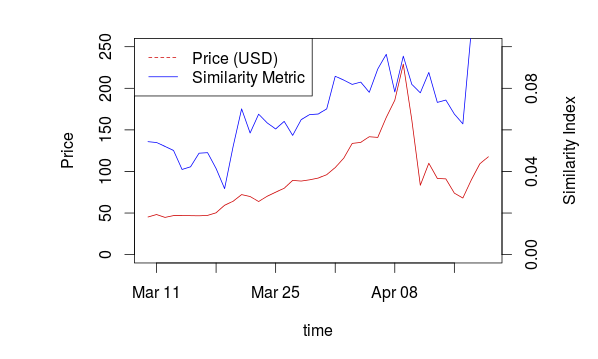
\includegraphics[width=\textwidth]{./Figures/pnc.png}
\caption{Daily transactions price correlation with network structure. The similarity index was calculated by RWGK }
\label{fig:RWGK}
\end{center}
\end{figure}

Although random walk kernels are still among the widely adopted graph kernels, one common disadvantage with them is that walks and paths do not capture information of the substructures present in the graph. The weak correlation as seen in the figure \ref{fig:RWGK} support our reasoning. Possibility of tottering \citep{Mahe2004} and halting \citep{Sugiyama2015} problem cannot be ruled out. This in turns focus our direction to use other graph kernels, free from above problem and can be scalable.

Next we use propagation kernels, whose design is motivated by the
iterative information propagation. They not only capture structural information, but can often adapt to the aforementioned issues of real world data. Adding to the same, they didn’t  suffer from the problem of halting and tottering \citep{Neumann2015}. Figure \ref{fig:PGK} plot the correlation between network structure and BTC/USD exchange price.

\begin{figure}[ht]
\begin{center}
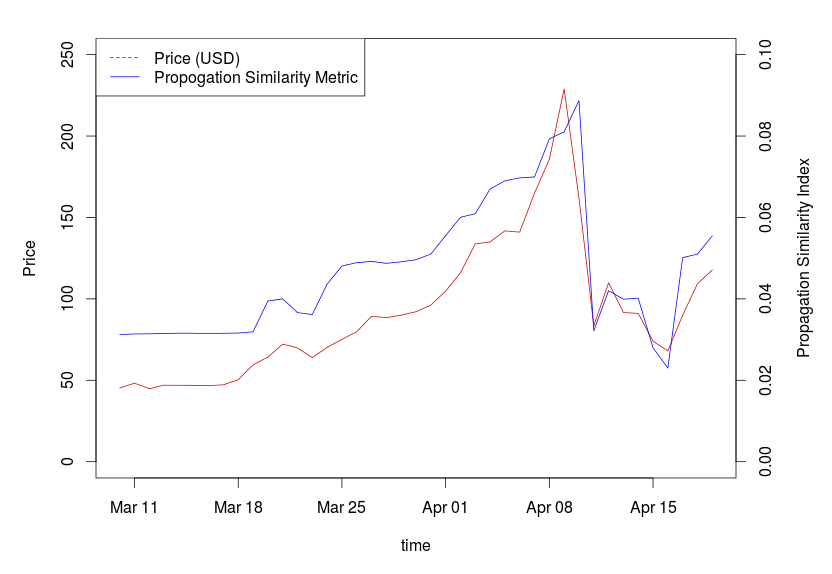
\includegraphics[width=\textwidth]{./Figures/PGK.png}
\caption{Daily transactions price correlation with network structure. The similarity index was calculated by PGK }
\label{fig:PGK}
\end{center}
\end{figure}

As expected figure \ref{fig:PGK} infer that the time-varying contribution of large scale transaction network correspondence with the market price of bitcoins, but there is still hope for the improvement, as graph is not smooth.
 

\section{Conclusions}

The purpose of this thesis is to offer an accurate and efficient similarity measure for dynamically changing large-scale graphs and structurally comparable graphs. By defining quantitative measure of transformation over time, in terms of similarity index using differnt kernels, we infer that there is correspondence between network structure and exchange price in bitcoin. The not so smooth graph direct our research to use other graph kernels. Our analysis of real-world transaction data from bitcoin  showcases a successful application of the method, which can further be employed in analyzing data from various fields.

\section{Summary}
This chapter review of representative graph kernels in the literature. By taking conventional and sophisticated graph kernels, this chapter defines   quantitative measure of transformation over time. The chapter concludes with not so smooth correspondence between network structure and exchange price in bitcoin, thus paving way for further investigation to other graph kernels.
%----------------------------------------------------------------------------------------
